\chapter{Testing}

\label{kap:testing} % id kapitoly pre prikaz ref
\paragraph*{}
This chapter displays results generated using our tool and compares them with results from similar programs. It also discusses the source of data used for comparison as well as settings used by individual programs.

\section{Source of data}
\paragraph*{}
For our tests to have any informative value, we need to know a large amount of information about the samples used. Since we did not possess samples with sufficient information, we decided to simulate our samples. We simulate our data using InSilicoSeq, a tool designed to generate simulated sequenced reads from sequences input by the user. The reads can be generated using either one of the pre-build error models or a custom model generated using a bam file with aligned reads. The pre-build error models include models for Illumina sequencers MiSeq, HiSeq, and NovaSeq.

To generate our samples, we use all three default error models. As the input sequences, we use a variable number of random phage genomes downloaded from NCBI. For our purposes, we used either ten or fifty genomes. We also adjust InSilicoSeq to generate one or five million reads per sample. We have decided that using other numbers of reads or genomes is redundant and thus do not use them. With these settings, we generate a total of twelve paired-end input samples.

\section{Settings}
\paragraph*{}
Aside from Phendol, we process the generated samples using multiPhATE and RASTtk. In this section, we describe the settings used for each tool.

\subsection{Phendol}
\paragraph*{}
We set Phendol to sample two million reads from the generated samples. This allows us to test Phendol on a full-sized dataset in case of the samples containing one million reads and test it on a sampled dataset when working with samples containing five million reads. We used 32 threads to run SPAdes. Contigs generated by SPAdes were later used in the analysis by other tools as well.

To test different setups of Phendol, we set the minimal percentage of identical matches in blast search to 75\% and 90\%. For the same reason, we set the minimum percentage of coverage of sequences from the endolysin database to 50\% and 75\%. We also made an analysis using values of 50\% for identity and 30\% for coverage.

The minimal length of endolysins was left at the default value of 40 amino acids. Finally, we sorted the output by the percentage of the sequence covered by hits from the database.

To reduce the runtime, we ran SPAdes only once per sample by manually copying its results into the working directories of other analyses. With these settings, we ran the pipeline five times per sample, resulting in a total of sixty analyses.

\subsection{multiPhATE}
\paragraph*{}
In the comparison, we use multiPhATE2, which is an enhanced version of multiPhATE. MultiPhATE uses a config file to specify all parameters. In the config file, we enabled the use of gene callers Phanotate, Prodigal, and Glimmer. We also enabled the blastp search. MultiPhATE has two default databases against which it can run the blastp search. These are Prokaryotic Virus Orthologous Groups (pVOGs) \cite{grazziotin2016prokaryotic} and The Phage Annotation Tools and Methods (PhAnToMe) database. In our setup, we use both.

We also set the list of genomes used in the analysis in the config file. In our case, the genomes set were the contigs produced by SPAdes during the run of Phendol. With the configuration complete, we ran multiPhATE to get the analyses for every sample.

\subsection{RASTtk}
\paragraph*{}
We attempted to install the command-line version of RASTtk, however, since the command-line version is outdated and not usable, we used the online browser version.

For the \texttt{create-genome} script, we set the domain as virus and the genetic code to 11 Archaea, most Bacteria, most Virii, and some Mitochondria). In our custom pipeline used for annotation, we use most of the scripts used in the default pipeline except for \texttt{call-strep-suis-repeat} and \texttt{call-strep-pneumo-repeat}, since the sequences we are annotating do not contain bacterial DNA. We also switch off the \texttt{resolve-overlapping-features} script because viral genomes tend to contain overlapping features.

We used this pipeline to analyse the contigs created by SPAdes during the run of Phendol.

\section{Comparison}
\paragraph*{}
In running RASTtk, we were unable to get results using the sample \texttt{50HiSeq1000000}. As a result, we only achieved results in the remaining eleven samples. In these results, we only counted the number of sequences directly designated by RASTtk as encoding endolysins, since the number of genes discovered with a less precise designation (e.g. Hypothetical protein) is impractically large and it is not feasible to verify them in the laboratory.

While running multiPhATE, we encountered several errors due to unknown reasons. This led to only analyses on samples \texttt{MiSeq} being completed. As with RASTtk, we only include sequences designated as encoding endolysins by multiPhATE directly.

Since the number of phages discovered by Phendol tended to vary between the number discovered with an identity of 75\% and coverage of 50\% and the number discovered with an identity of 90\% and coverage of 75\%, we do not include other combinations of these values in our comparison. We also filter the results of the analysis with identity set to 50\% and coverage 30\% because the unfiltered result contains a large number of sequences with a low probability of being an endolysin. We consider sequence as having a low probability of being an endolysin when the coverage of the sequence by Blast hits is lower than 50\%. In the comparison, we include both the filtered and unfiltered analysis.

When comparing the results, we decided to base our ground truth on the number of genomes included in each sample. In doing so, we assume that every phage genome contains at least one endolysin encoding gene to facilitate its ability to complete its lytic cycle. We also assume that every phage genome contains at most one endolysin encoding gene. In our comparison, we prefer false positives to false negatives. We make this preference because the false positives can be further verified in wet-lab while the false negatives cannot be restored. As a result, our ground truth is ten for analyses done on samples containing ten genomes and fifty for analyses done on samples with fifty genomes.

\begin{figure}[h]
  \begin{center}
     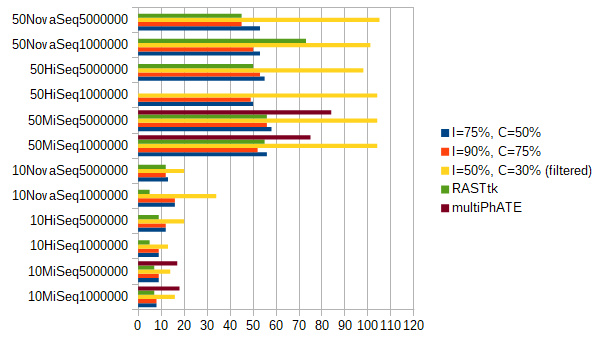
\includegraphics[width=0.9\textwidth]{images/results.png}
     \caption{Number of predicted endolysins per sample by analysis method.}\label{fig:results}
  \end{center}
\end{figure} 

Compared with RASTtk, Phendol was generally capable of annotating a larger number of endolysins, with the filtered analysis predicting a significantly higher number of endolysins (Figure \ref{fig:results}). 

When compared with multiPhATE, Phendol discovered mostly a lower number of endolysins while being closer to our ground truth (Figure \ref{fig:results}). The only exception was the filtered analysis, which predicted a similar or higher number of endolysins.

In comparison with both RASTtk and multiPhATE, the predictions made by Phendol with identity between 75-90\% and coverage between 50-75\% were closer to our ground truth making Phendol more accurate. By decreasing the identity and coverage Phendol has the option of decreasing the number of false negatives at the cost of an increase in the number of false positives. This exchange is advisable in order to discover endolysins more thoroughly as it facilitates more wet-lab verification.
